This section describes shortly how the Cristin API was implemented. It then describes the process of crawling Cristins RDBMS. Finally, it describes how the extracted data was processed to create relations and nodes in a graph database.

% Skakke ha kake a kai
% Skrive en liten del om hvordan en henter ut data fra CRISTIN sitt API.
%	Rationale: Muliggjøre at en leser skal kunne reimplementere det vi har gjort
\subsection*{Cristin API}
Cristin provides APIs to extract information by querying a REST or Web Service API, which results in queries to the underlying RDBMS with more or less processing depending on the API buing used and endpoint queried\cite{CRISTIN-API-summary}.

The Web Service API\cite{CRISTIN-WS} is still available for legacy purposes, and enable querying for scientific results by a particular person. This functionality is not available in the more modern REST API. The REST API\cite{CRISTIN-REST} allow queries with less processing on the server's side than the Web Service API, but without the ability to query scientific results, such as papers in journals and presentations at conferences.

All data discussed later in the paper is extracted through these API's.

\subsection*{Crawling Cristin}
Authors are stored with ID's starting from 0, but with a large number of vacant person ID's, and the importance of relationship, makes rearching persons with monotonically increasing person ID infeasible.
Due to this limitation, a crawler is implemented. It will start at a person, retrieve the scientific results of that person, mark that person as crawled, store the results, and crawl each of the collaborating authors for all results retrieved that have not already been crawled, as to eliminate crawling cycles.
The number of authors to crawl will grow exponentially until all authors are finally crawled.

\subsection*{Processing extracted data}
Data extracted from Cristin is structured in json format which makes it easy to work with. Json objects are a key-value store which makes it similar to nodes in a graph database. Nodes are the entities in a graph database. They can hold any number of attributes (key-value-pairs) called properties. Nodes can be tagged with labels representing their different roles in your domain.\cite{neo4j} The difference between a json object and a node is that a json value can take form of a \textit{dictionary} and a property value can't. A json object is compatible as a node if none of the values are a dictionary and a label is attached to it.

\subsection*{Inserting data}
Inserting nodes into a graph database is straight forward, but creating relations between nodes can be a hassle. The challange is to know wether two nodes exists in the database before creating a relationship between them. \Fref{fig:subgraph} shows that the relationship \textit{guest} can't be created unless the green \textit{unit} node, red \textit{institution} node and the blue \textit{person} node exists in the database.

\begin{figure}[h]
  \centering
  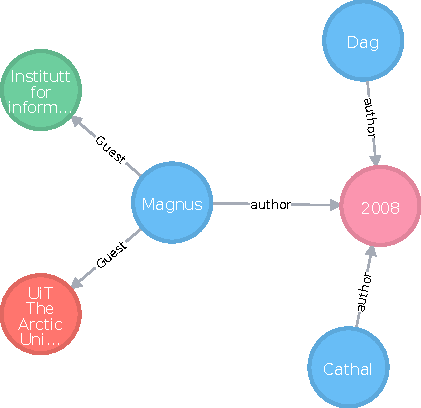
\includegraphics[width=0.35\textwidth]{graph.pdf}
  \caption{A subgraph}
  \label{fig:subgraph}
\end{figure}


% Kákékúngen
% Kanskje en idé å nevne terminologien vi bruker. (?)
% Hvor passer dette best?
\subsection*{Exploring data}
As previously mentioned, the goal of this paper is to show how people in the scientific community collaborate across units within the same institutions as well as across different institutions.
This can easily be modeled by using a graph database and the queries themselves as graph traversals.
We will argue both for the performance and for the ergonomy of the graph model provided by Neo4j over a RDBMS.
